The Vortex Æther Model (VAM), developed by O. Iskandarani since 2012, models the æther as an incompressible, non-viscous superfluid~\cite{VAM-8, VAM-13}. Within this framework, vorticity is elevated to a fundamental quantity that governs time dilation, inertial mass, and gravitational interaction~\cite{VAM-2, VAM-10, VAM-13}. Echoing Einstein’s 1920 redefinition of the æther as a physical substratum, VAM treats the æther as a structured, causal medium from which all dynamical behavior emerges~\cite{VAM-8}.

Key structural elements of VAM include:
\begin{itemize}
    \item \textbf{Topological structures} (e.g., knots, trefoils) representing stable particle identities and quantum numbers~\cite{VAM-8, VAM-11, VAM-14},
    \item \textbf{Time dilation} arising from swirl intensity near vortex cores~\cite{VAM-2, VAM-13},
    \item \textbf{A revised system of natural constants}, including $C_e$ (vortex boundary velocity) and $F^{\max}_{\text{\ae}}$ (maximum ætheric stress), defined and operationalized in the topological Lagrangian~\cite{VAM-14}.
\end{itemize}

Figure~\ref{fig:taxonomy} illustrates the classification flow based on topology, chirality, and tension within the swirl field framework.


\begin{figure}[!ht]
    \centering
    \footnotesize
    \scalebox{0.75}{
        \begin{tikzpicture}[
          box/.style = {draw, rounded corners, minimum width=2.0cm, minimum height=0.8cm, font=\small, align=center},
          arrow/.style = {->, thick},   node distance=1.0cm and 1.5cm
        ]
            % Inputs
            \node[box] (topology) {Knot Topology};
            \node[box, right=of topology] (chirality) {Chirality};
            \node[box, right=of chirality] (tension) {Tension};

            % Swirl coupling
            \node[box, below=of chirality, minimum width=5.5cm] (coupling) {Swirl Coupling Condition};

            % Gravitational response
            \node[box, below=of coupling] (grav) {Gravitational Response};

            % Gravitational classes
            \node[box, below left=1.3cm and 1.5cm of grav] (matter) {Chiral\\Leptons \& Quarks};
            \node[box, below=2cm of grav] (boson) {Achiral + No Tension\\\(\rightarrow\) Bosons};
            \node[box, below right=1.3cm and 1.7cm of grav] (dark) {Achiral + Tension\\\(\rightarrow\) Dark Energy Knots};

            % Subclasses
            \node[box, below=of matter, xshift=-1.5cm] (leptons) {Leptons\\(e\textsuperscript{--} = T(2,3))};
            \node[box, below=of matter, xshift=+1.0cm] (quarks) {Quarks\\(6\textsubscript{2}, 7\textsubscript{4}, 8\textsubscript{19})};

            \node[box, below=of boson, xshift=-2.1cm] (photon) {Photon\\(unknot)};
            \node[box, below=of boson] (gluon) {Gluon\\(Hopf link)};
            \node[box, below=of boson, xshift=+2.3cm] (zboson) {Z\textsuperscript{0}\\(neutral loop)};

            \node[box, below=of dark] (darkex) {Example: \(4_{1}, 8_{17}\)\\ (achiral hyperbolic)};

            % Arrows to coupling
            \draw[arrow] (topology.south) -- ++(0,-0.5) -| (coupling.north west);
            \draw[arrow] (chirality.south) -- (coupling.north);
            \draw[arrow] (tension.south) -- ++(0,-0.5) -| (coupling.north east);

            % Arrows down flow
            \draw[arrow] (coupling.south) -- (grav.north);
            \draw[arrow] (grav.south) -- (matter.north);
            \draw[arrow] (grav.south) -- (boson.north);
            \draw[arrow] (grav.south) -- (dark.north);

            % Particle branches
            \draw[arrow] (matter.south) -- (leptons.north);
            \draw[arrow] (matter.south) -- (quarks.north);

            \draw[arrow] (boson.south) -- (photon.north);
            \draw[arrow] (boson.south) -- (gluon.north);
            \draw[arrow] (boson.south) -- (zboson.north);

            \draw[arrow] (dark.south) -- (darkex.north);
        \end{tikzpicture}
    }
    \caption{
        \textbf{Knot Classification by Swirl Coupling.}
        This flow diagram illustrates how fundamental particle types in the VAM framework emerge from topological features of vortex knots. (See classification list below.)
    }
    \label{fig:taxonomy}

\end{figure}

\vspace{0.1em}
\textbf{Classification summary:}
Knot topology, chirality, and curvature tension collectively determine a knot’s gravitational and inertial response, enabling classification into Standard Model families:
\begin{itemize}
    \item \textbf{Chiral knots} align with swirl fields and give rise to matter: \textbf{Leptons} (e.g., torus knots like \( T(2,3) \)), \textbf{Quarks} (e.g., hyperbolic knots like \( 5_2, 6_1, 8_{19} \)).
    \item \textbf{Achiral, tensionless} structures (unknots, Hopf links): \textbf{bosons}.
    \item \textbf{Achiral knots with intrinsic tension}: expelled, possible \textbf{dark energy} candidates (\( 4_1, 8_{17} \)).
\end{itemize}
\vspace{0.3em}

The classification is governed by the Swirl Coupling Condition, connecting geometric knot invariants to physical properties such as mass, spin, and interaction profile.

Knot theory has long informed fluid dynamics and topological invariants in vorticity~\cite{knot_theroy_in_fluid}, providing a mathematical foundation for the VAM taxonomy of particles as stable knotted structures.

\subsection*{Wave–Particle Duality Reconsidered}

The historical tension between wave and particle descriptions has long shaped the conceptual foundations of physics. From Democritus’s indivisible atoms to Newton’s corpuscular optics and Huygens’s wave theory, the debate culminated in quantum mechanics with the paradoxical coexistence of wavefunctions and discrete quanta.

In the Vortex Æther Model (VAM), this duality is resolved not as a fundamental contradiction, but as an artifact of interpreting structured vortex excitations within an underlying fluid medium. Particles are modeled as knotted, topologically stable vorticity configurations, whose wave-like behavior emerges naturally from interference, circulation, and swirl-phase dynamics in the æther—eliminating the need for a dual ontology.

Figure~\ref{fig:WaveParticleDuality} situates this resolution within the broader intellectual trajectory of wave–particle theory—tracing its evolution from ancient atomism and early wave optics to modern quantum mechanics and finally the unified vortex framework offered by VAM.


\resizebox{\textwidth}{!}{%
      \centering
    \scriptsize
    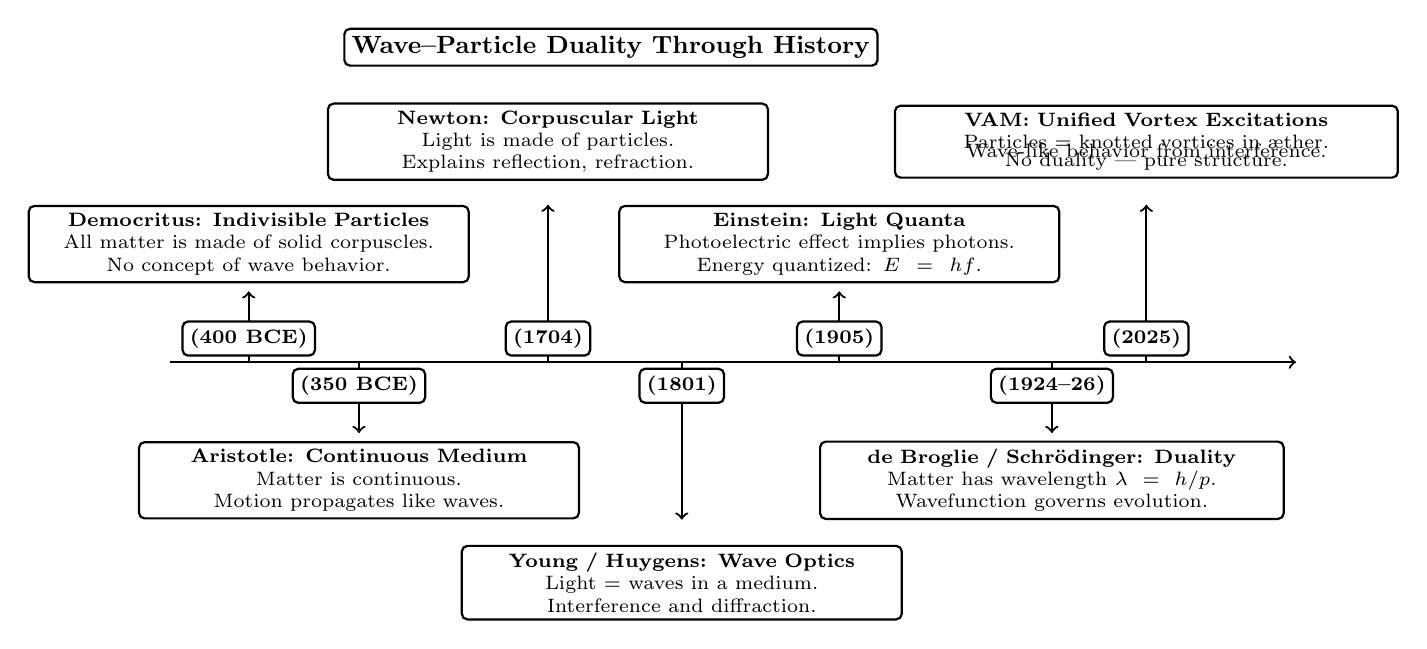
\begin{tikzpicture}
    \scriptsize

    % Timeline base
    \draw[->, thick] (-1,0) -- (13.3,0);

    % Arrows above timeline
    \draw[->, thick] (0,0) -- (0,0.9);       % Democritus
    \draw[->, thick] (3.8,0) -- (3.8,2.0);   % Newton
    \draw[->, thick] (7.5,0) -- (7.5,0.9);   % Einstein
    \draw[->, thick] (11.4,0) -- (11.4,2.0); % VAM

    % Arrows below timeline
    \draw[->, thick] (1.4,0) -- (1.4,-0.9);     % Aristotle
    \draw[->, thick] (5.5,0) -- (5.5,-2.0);     % Young/Huygens
    \draw[->, thick] (10.2,0) -- (10.2,-0.9);   % de Broglie

    % --- Date labels ---
    \node[draw, thick, rounded corners=2pt, fill=white, align=center, font=\bfseries ] at (0, .3)   {(400 BCE)};
    \node[draw, thick, rounded corners=2pt, fill=white, align=center, font=\bfseries ] at (3.8, .3) {(1704)};
    \node[draw, thick, rounded corners=2pt, fill=white, align=center, font=\bfseries ] at (7.5, .3) {(1905)};
    \node[draw, thick, rounded corners=2pt, fill=white, align=center, font=\bfseries ] at (11.4, .3){(2025)};

    \node[draw, thick, rounded corners=2pt, fill=white, align=center, font=\bfseries ] at (1.4,- .3) {(350 BCE)};
    \node[draw, thick, rounded corners=2pt, fill=white, align=center, font=\bfseries ] at (5.5,- .3) {(1801)};
    \node[draw, thick, rounded corners=2pt, fill=white, align=center, font=\bfseries ] at (10.2,- .3) {(1924--26)};

    % Timeline label
    \node[draw, thick, fill=white, rounded corners=2pt, font=\small] at (4.6,4.0) {\textbf{Wave–Particle Duality Through History}};

    % --- Democritus ---
    \node[draw, rounded corners=2pt, thick, align=center, fill=white, text width=5.4cm] at (0,1.5) {
    \textbf{Democritus: Indivisible Particles} \\% [-0.8em]
    All matter is made of solid corpuscles. \\% [-0.8em]
    No concept of wave behavior.
    };

    % --- Newton ---
    \node[draw, rounded corners=2pt, thick, align=center, fill=white, text width=5.4cm] at (3.8,2.8) {
    \textbf{Newton: Corpuscular Light} \\% [-0.8em]
    Light is made of particles. \\% [-0.8em]
    Explains reflection, refraction.
    };

    % --- Einstein ---
    \node[draw, rounded corners=2pt, thick, align=center, fill=white, text width=5.4cm] at (7.5,1.5) {
    \textbf{Einstein: Light Quanta} \\% [-0.8em]
    Photoelectric effect implies photons. \\% [-0.8em]
    Energy quantized: \( E = hf \).
    };

    % --- VAM ---
    \node[draw, rounded corners=2pt, thick, align=center, fill=white, text width=6.2cm] at (11.4,2.8) {
    \textbf{VAM: Unified Vortex Excitations} \\% [-0.8em]
    Particles = knotted vortices in æther. \\[-0.6em]
    Wave-like behavior from interference. \\[-0.6em]
    No duality — pure structure.
    };

    % --- Aristotle ---
    \node[draw, rounded corners=2pt, thick, align=center, fill=white, text width=5.4cm] at (1.4,-1.5) {
    \textbf{Aristotle: Continuous Medium} \\% [-0.8em]
    Matter is continuous. \\% [-0.8em]
    Motion propagates like waves.
    };

    % --- Young / Huygens ---
    \node[draw, rounded corners=2pt, thick, align=center, fill=white, text width=5.4cm] at (5.5,-2.8) {
    \textbf{Young / Huygens: Wave Optics} \\% [-0.8em]
    Light = waves in a medium. \\% [-0.8em]
    Interference and diffraction.
    };

    % --- de Broglie / Schrödinger ---
    \node[draw, rounded corners=2pt, thick, align=center, fill=white, text width=5.7cm] at (10.2,-1.5) {
    \textbf{de Broglie / Schrödinger: Duality} \\% [-0.8em]
    Matter has wavelength \( \lambda = h/p \). \\% [-0.8em]
    Wavefunction governs evolution.
    };

    \end{tikzpicture}
    \caption{\textbf{Intellectual trajectory of wave–particle duality:} from classical corpuscles and wave models to quantum dualities and beyond. VAM reframes the dichotomy by modeling all excitations as topologically structured vortices in a fluid æther. In this view, “particles” and “waves” are unified as geometric flow phenomena—dispensing with dualism in favor of pure structure.}\label{fig:WaveParticleDuality}
}


\subsection*[VAM-Derived Expression for G]{VAM-Derived Expression for G}

One of the notable results in VAM is a derivation of the gravitational constant in terms of ætheric and topological parameters~\cite{VAM-2, VAM-13, VAM-14}. Rewriting the expression in dimensionally transparent form:

\begin{equation}
    G_\text{swirl} = \frac{C_e}{2 F^{\max}_{\text{\ae}}} \cdot \left( \frac{c^5 t_p^2}{r_c^2} \right)
\end{equation}

\noindent where:
\begin{itemize}
    \item $C_e$: swirl velocity at the vortex boundary (m/s),
    \item $F^{\max}_{\text{\ae}}$: maximum force the æther can sustain before bifurcation (N),
    \item $t_p$: Planck time $ \left(\sqrt{\hbar G / c^5}\right) $,
    \item $r_c$: core radius of the vortex structure (m),
    \item $c$: speed of light in vacuum (m/s).
\end{itemize}

This formulation emerges from the Swirl Clock formalism and connects gravity to rotational energy density under conservation of circulation~
\cite{VAM-2, VAM-13}. It expresses $G$ not as a fundamental input constant, but as a derived quantity arising from the interplay of topological scale~\cite{bartini2005constants} $r_c$, rotational dynamics $C_e$, and ætheric tension $F^{\max}_{\text{\ae}}$. This reinforces the view that gravitation is a residual effect of conserved vorticity in a compressible ætheric medium. This formulation echoes recent emergent gravity approaches~\cite{Verlinde2011,Hossenfelder2017}, yet grounds gravity not in entropic gradients but in rotational conservation and swirl tension, which resonates with dynamical 3-space theories, in which gravity emerges from self-interacting spatial flow~\cite{cahill2003dynamical}.

VAM further incorporates circulation quantization, helicity conservation, and pressure-mediated interactions to model the exchange between knotted structures and their surrounding swirl fields~\cite{VAM-8, VAM-11, VAM-14}, consistent with nonlinear wave-vortex interaction theory in rotating fluids~\cite{buhler2005wave}. This general framework aligns with Einstein’s late attempt at a unified field theory—now realized through the mathematics of topological fluid dynamics.

The model's predictions are experimentally approachable through analog systems such as rotating superfluid vortices, BEC interference patterns, and refractive index shifts under swirl acceleration~\cite{VAM-2, VAM-13}. Such analogs mirror behavior seen in superfluid helium systems, including vortex quantization and phase discontinuities~\cite{tilley_superfluid}.  These offer testable pathways for validating the core dynamics proposed by VAM. These dynamics have observable analogs in superfluid and BEC systems, as described in analogue gravity programs~\cite{barcelo2005}.


\vspace{1em}